\chapter{Results}
This chapter shows the results of the experiment and how the gathered data can be interpreted. 


\subsection{output format}
Figure \ref{entries} shows how the gathered data look after the decryption. 

\begin{figure}[!htb]
\centering
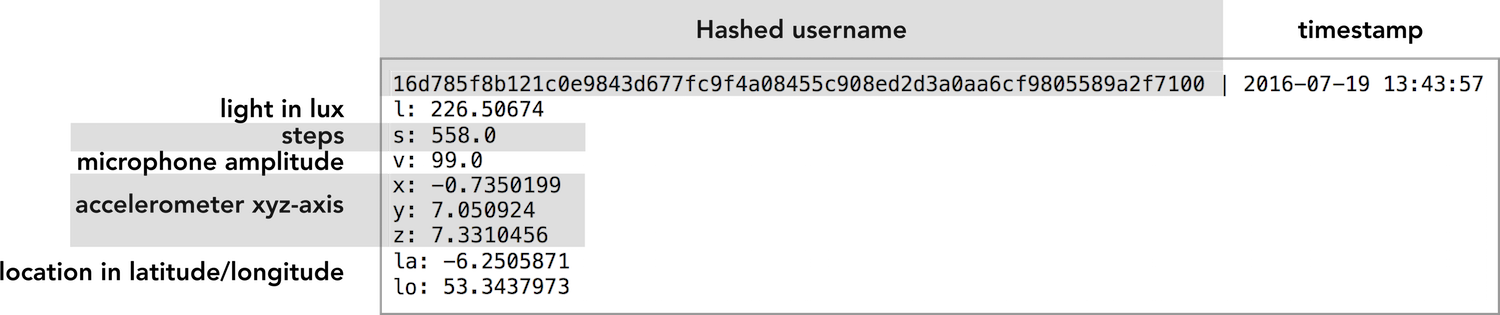
\includegraphics[width=\textwidth]{entries}
\caption{gathered data}\label{entries}
\vspace{10 mm}
\end{figure}

\FloatBarrier

\bigbreak

Participant number 2 was the only one who answered the question of being distracted during the experiment with 'yes'. Also the volume amplitude had some very high peeks that were not found in the measurements of other participants in that level. The distracted participant also needed to longest to solve the programming task \ref{volps}. 

\subsection{Volume}
\begin{figure}[ht]
	\centering
	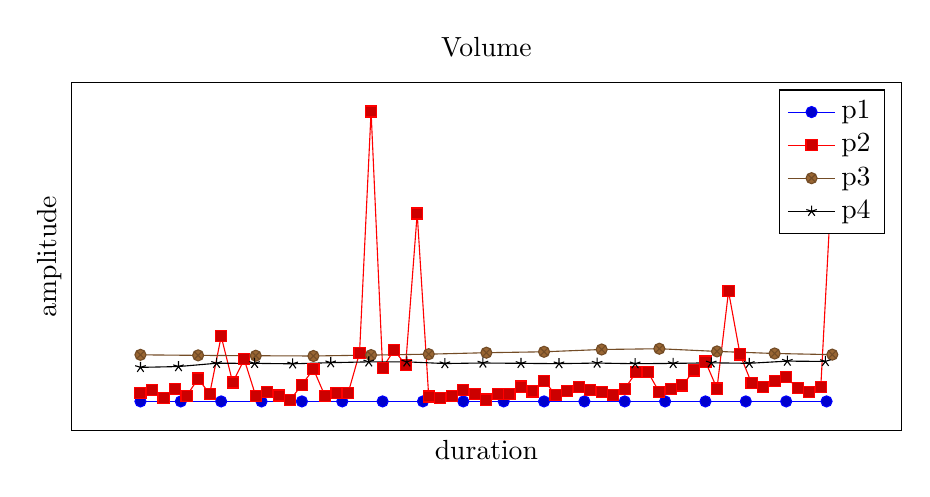
\begin{tikzpicture}
	\pgfplotsset{ticks=none}
\begin{axis}[
	height=6cm,
	width=\textwidth,
	ylabel=amplitude,
	xlabel=duration,
	title=Volume,
	unbounded coords=discard],
	
\addplot coordinates {
(0, 0.0)
(3.5, 0.0)
(7, 0.0)
(10.5, 0.0)
(14, 0.0)
(17.5, 0.0)
(21, 0.0)
(24.5, 0.0)
(28, 0.0)
(31.5, 0.0)
(35, 0.0)
(38.5, 0.0)
(42, 0.0)
(45.5, 0.0)
(49, 0.0)
(52.5, 0.0)
(56, 0.0)
(59.5, 0.0)
};

\addplot coordinates {
(0 , 59.5882352941)
(1 , 83.125)
(2 , 23.0)
(3 , 88.25)
(4 , 38.75)
(5 , 162.333333333)
(6 , 53.0)
(7 , 462.666666667)
(8 , 134.333333333)
(9 , 298.5)
(10 , 38.5)
(11 , 64.3333333333)
(12 , 42.0)
(13 , 12.5)
(14 , 117.75)
(15 , 229.5)
(16 , 39.6666666667)
(17 , 57.0)
(18 , 57.0)
(19 , 344.333333333)
(20 , 2060.0)
(21 , 238.6)
(22 , 365.0)
(23 , 259.0)
(24 , 1335.16666667)
(25 , 35.0)
(26 , 24.0)
(27 , 39.3333333333)
(28 , 80.0)
(29 , 52.0)
(30 , 13.25)
(31 , 52.3333333333)
(32 , 50.75)
(33 , 105.5)
(34 , 70.75)
(35 , 147.666666667)
(36 , 47.0)
(37 , 76.5)
(38 , 104.0)
(39 , 80.8)
(40 , 69.0)
(41 , 45.1666666667)
(42 , 90.3333333333)
(43 , 208.0)
(44 , 210.0)
(45 , 65.3333333333)
(46 , 86.5)
(47 , 113.25)
(48 , 220.0)
(49 , 283.0)
(50 , 91.5)
(51 , 782.0)
(52 , 333.666666667)
(53 , 129.333333333)
(54 , 102.0)
(55 , 145.0)
(56 , 171.0)
(57 , 93.5789473684)
(58 , 68.75)
(59 , 100.0)
(60 , 1637.83333333)
};

\addplot coordinates {
(0 , 330.986057143)
(5 , 327.141866667)
(10 , 324.539771429)
(15 , 322.701066667)
(20 , 329.208342857)
(25 , 335.669942857)
(30 , 346.047466667)
(35 , 352.541066667)
(40 , 368.9453)
(45 , 374.263066667)
(50 , 355.196133333)
(55 , 340.515885714)
(60 , 332.4064)
};

\addplot coordinates {
(0, 241.869565217)
(3.3, 247.684210526)
(6.6, 271.19047619)
(9.9, 270.380952381)
(13.2, 267.19047619)
(16.5, 275.181818182)
(19.8, 281.0)
(23.1, 281.0)
(26.4, 269.056565454)
(29.7, 273.082245)
(33, 270.457685359)
(36.3, 268.358045125)
(39.6, 272.456782138)
(42.9, 268.0)
(46.2, 270.121246868)
(49.5, 274.154865478)
(52.8, 270.782398425)
(56.1, 286.252546845)
(59.4, 284.054086785)
};

\addlegendentry{p1}
\addlegendentry{p2}
\addlegendentry{p3}
\addlegendentry{p4}
\end{axis}

\end{tikzpicture}
\caption{Noise Participants}\label{volps}
 	\vspace{5 mm}
\end{figure}

\FloatBarrier

\section{Individual Experiment Results}
The results of the individual experiment are demonstrating the usage and the abilities for the Dather Application for a single participant. Rather than in the first experiment, it is taking only the data of a single person into account.
The data is only a trend but not a scientific result. A lot more test cases would be needed to create a more accurate average value. However, the purpose of this experiment was to demonstrate the usage of the data, more to create comparable environments rather than in experiment number 1 detect the environment and patterns. 

\subsection{coffee}
The table \ref{coffee} shows the times of 10 Sudoku solvings of the participant. The results show that at the beginning, the participant was faster under the influence of caffeine and then later on the opposite. As the measurements where done on different days, the participant probably gained more practice in solving Sodukus, which shows the decreasing time to solve a Sudoku.
\\
The average time, the participant needed without drinking coffee was \textbf{14:24 minutes} and after consuming \textbf{17:37 minutes} minutes per Sudoku. The participnat needed 3:13 minutes or 22.34\%  longer after having a strong coffee \ref{resultCoffee}.\\
These results are different than the findings in \cite{liguori1997absorption}. Their results showed that a similar amount of caffeine increases the cognitive performance. \\
However, in our case the participant of the Experiment mentioned to feel fretful after the intake of the high amount of caffeine. That could be a reason for the lower performance of the subject. Thus, it is possible that a overdose had negative impact on the participant and lower amount of caffeine would have had resulted better. 

\FloatBarrier

%%%% Coffee times
\setlength{\tabcolsep}{10pt}
\renewcommand{\arraystretch}{1.5}
{\rowcolors{3}{black!10!white!90}{white!100}

\begin{table}[!htb]
\centering
\begin{adjustbox}{width=1\textwidth}
\begin{tabular}{ |p{2,5cm}|P{0.8cm}|P{0.8cm}|P{0.8cm}|P{0.8cm}|P{0.8cm}|P{0.8cm}|P{0.8cm}|P{0.8cm}|P{0.8cm}|P{0.8cm}|  }
 \hline
 \rowcolor{lightgray} \multicolumn{11}{|c|}{{\bf Experiment with Caffeine}} \\
 \hline
 \hline
  {Condition}
   & \multicolumn{10}{|c|}{Duration} \\
    \cline{2-11}
    \hline
 \hline
 Measurement	& 1			& 2			& 3			& 4			& 5			& 6 			& 7 			& 8 			& 9			& 10			\\
 No Coffee		& 20:43	& 21:36	& 13:14	& 23:02	& 09:32	& 12:18 	& 15:05 	& 09:49 	& 10:07	& 08:41	\\
 Coffee   			& 12:39	& 22:32	& 09:00 	& 26:34 	& 14:23	& 16:21	& 25:18	& 16:16	& 14:47	& 18:15	\\
 \hline
\end{tabular}
\end{adjustbox}
\caption{Cognitive Performance with Coffee}
\label{coffee}
\end{table}


% Define bar chart colors
%
\definecolor{noCoff}{HTML}{1c90e7}
\definecolor{coffee}{HTML}{a4c639}

\begin{figure}
	\centering
	\begin{tikzpicture}
        \begin{axis}[
            width  = 0.5*\textwidth,
        	height = 8cm,
        	major x tick style = transparent,
        	ybar=2*\pgflinewidth,
        	bar width=30pt,
        	ymajorgrids = true,
        	ylabel = {Average solving time},
        	symbolic x coords={Influences},
       	 	xtick = data,
        	scaled y ticks = false,
        	enlarge x limits=0.25,
        	ymin=0,
        	legend cell align=left,
        	legend style={
                at={(1,1.05)},
                anchor=south east,
                column sep=1ex
        	}
      	]
     	\addplot[style={android,fill=noCoff,mark=no coffee}]
            coordinates {(Influences, 14.04)};

        \addplot[style={ios,fill=coffee,mark=coffee}]
             coordinates {(Influences,18.25)};

        \legend{No Coffee, Coffee} 

        \end{axis}
 	\end{tikzpicture}
 	\caption{Solving times - Coffee} \label{resultCoffee}
 	\vspace{10 mm}
\end{figure}

\FloatBarrier

\subsection{music}

The table \ref{music} shows the times of the Sudokus that have been solved by the participant and the duration it took. It shows that the average time of solving was the shortest when the participant was listening to music. 
The participant solved the ten Sudokus in 89.35\% of the average time compared to the results archived without music. That is 1 minute and 34 seconds less time in average. 
On the other hand, the average solving time while listening to heavy metal music was 4.08 \% or 36 seconds slower than without listening to music. 
The results show evidence that for the participant the cognitive performance in solving Sudoku riddles was increasing when listening to classical music and decreasing at heavy metal music. 

\FloatBarrier

%%%% Music times
\setlength{\tabcolsep}{10pt}
\renewcommand{\arraystretch}{1.5}
{\rowcolors{3}{black!10!white!90}{white!100}

\begin{table}[!htb]
\centering
\begin{adjustbox}{width=1\textwidth}
\begin{tabular}{ |p{2,5cm}|P{0.8cm}|P{0.8cm}|P{0.8cm}|P{0.8cm}|P{0.8cm}|P{0.8cm}|P{0.8cm}|P{0.8cm}|P{0.8cm}|P{0.8cm}|  }
 \hline
 \rowcolor{lightgray} \multicolumn{11}{|c|}{{\bf Experiment with Music}} \\
 \hline
 \hline
  {Condition}
   & \multicolumn{10}{|c|}{Duration} \\
    \cline{2-11}
    \hline
 \hline
 Measurement	& 1			& 2			& 3			& 4			& 5			& 6 			& 7 			& 8 			& 9			& 10			\\
 No Music			& 13:40	& 12:16	& 09:11	& 11:07	& 15:19	& 09:47	& 11:32	& 09:08	& 16:00	& 23:33	\\
 Heavy Metal   	& 30:12	& 15:51	& 14:42	& 15:46	& 19:47	& 09:51	& 11:01	& 12:34	& 09:58	& 13:23	\\
 Classical   		& 20:52	& 09:45	& 21:14	& 13:01	& 09:06	& 19:34	& 08:02	& 10:36	& 19:58	& 15:03	\\
 \hline
\end{tabular}
\end{adjustbox}
\caption{Cognitive Performance with Music}
\label{music}
\end{table}

% Define bar chart colors
%
\definecolor{nada}{HTML}{e78d1c}
\definecolor{metal}{HTML}{a4c639}
\definecolor{classical}{HTML}{1c90e7}

\begin{figure}
	\centering
	\begin{tikzpicture}
        \begin{axis}[
            width  = 0.5*\textwidth,
        	height = 8cm,
        	major x tick style = transparent,
        	ybar=2*\pgflinewidth,
        	bar width=30pt,
        	ymajorgrids = true,
        	ylabel = {Average solving time},
        	symbolic x coords={Influences},
       	 	xtick = data,
        	scaled y ticks = false,
        	enlarge x limits=0.25,
        	ymin=0,
        	legend cell align=left,
        	legend style={
                at={(1,1.05)},
                anchor=south east,
                column sep=1ex
        	}
      	]
     	\addplot[style={android,fill=classical,mark=classical}]
            coordinates {(Influences, 13.15)};

        \addplot[style={ios,fill=,metal,mark=metal}]
             coordinates {(Influences,15.316667)};

        \addplot[style={others,fill=nada,mark=no music}]
             coordinates {(Influences, 15.005)};

        \legend{Classical, Metal, No Music} 

        \end{axis}
 	\end{tikzpicture}
 	\caption{Solving times - Music}\label{resultMusic}
 	\vspace{10 mm}
\end{figure}

\FloatBarrier

